\chapter{Linear Equations} % Replace X with the chapter number and title

In this chapter, you will learn to:

\begin{enumerate}
    \item Graph a linear equation.
    \item Find the slope of a line.
    \item Determine an equation of a line.
    \item Solve linear systems.
    \item Do application problems using linear equations.
\end{enumerate}

\section{Graphing a Linear Equation}

In this section, you will learn to:

\begin{enumerate}
    \item Graph a line when you know its equation.
    \item Graph a line when you are given its equation in parametric form.
    \item Graph and find equations of vertical and horizontal lines.
\end{enumerate}

\subsection{Graphing a Line from its Equation}

Equations whose graphs are straight lines are called linear equations. The following are some examples of linear equations:

\begin{align*}
2x - 3y &= 6, \\
3x &= 4y - 7, \\
y &= 2x - 5, \\
2y &= 3, \\
x - 2 &= 0.
\end{align*}

A line is completely determined by two points. Therefore, to graph a linear equation, we need to find the coordinates of two points. This can be accomplished by choosing an arbitrary value for x or y and then solving for the other variable.

\begin{example}
Graph the line \(y = 3x + 2\).
\end{example}

\begin{solution} We need to find the coordinates of at least two points. We arbitrarily choose \(x = -1\), \(x = 0\), and \(x = 1\).

If \(x = -1\), then \(y = 3(-1) + 2\) or \(y = -1\). Therefore, \((-1, -1)\) is a point on this line.

If \(x = 0\), then \(y = 3(0) + 2\) or \(y = 2\). Hence the point \((0, 2)\).

If \(x = 1\), then \(y = 5\), and we get the point \((1, 5)\). Below, the results are summarized, and the line is graphed.

\begin{center}
\begin{tabular}{c|c}
    \(x\) & \(y\) \\
    \hline
    -1 & -1 \\
    0  & 2  \\
    1  & 5
\end{tabular}
\end{center}

% TODO add graphic here
\end{solution}

\begin{example}
Graph the line: $2x + y = 4$
\end{example}

\begin{solution} Again, we need to find coordinates of at least two points. We arbitrarily choose $x = -1$, $x = 0$, and $y = 2$.

If $x = -1$, then $2(-1) + y = 4$ which results in $y = 6$. Therefore, $(-1, 6)$ is a point on this line.

If $x = 0$, then $2(0) + y = 4$, which results in $y = 4$. Hence the point $(0, 4)$.

If $y = 2$, then $2x + 2 = 4$, which yields $x = 1$, and gives the point $(1, 2)$. The table below shows the points, and the line is graphed.

% TODO add graphic here

\begin{center}
\begin{tabular}{c|c}
    $x$ & $y$ \\
    \hline
    $-1$ & $6$ \\
    $0$  & $4$ \\
    $1$  & $2$
\end{tabular}
\end{center}
\end{solution}

\subsection{Intercepts:} The points at which a line crosses the coordinate axes are called the intercepts. When graphing a line by plotting two points, using the intercepts is often preferred because they are easy to find.
\begin{itemize}
    \item To find the value of the x-intercept, we let $y = 0$.
    \item To find the value of the y-intercept, we let $x = 0$.
\end{itemize}

\begin{example}
Find the intercepts of the line: $2x - 3y = 6$, and graph.
\end{example}

\begin{solution} To find the x-intercept, let $y = 0$ in the equation, and solve for $x$.
\begin{align*}
2x - 3(0) &= 6 \\
2x &= 6 \\
x &= 3
\end{align*}
Therefore, the x-intercept is the point $(3, 0)$.

To find the y-intercept, let $x = 0$ in the equation, and solve for $y$.
\begin{align*}
2(0) - 3y &= 6 \\
0 - 3y &= 6 \\
-3y &= 6 \\
y &= -2
\end{align*}
Therefore, the y-intercept is the point $(0, -2)$.

To graph the line, plot the points for the x-intercept $(3, 0)$ and the y-intercept $(0, -2)$, and use them to draw the line.

% TODO add graphic here
\end{solution}
\subsection{Graphing a Line from Its Equation in Parametric Form}

In higher math, equations of lines are sometimes written in parametric form. For example, $x = 3 + 2t, y = 1 + t$. The letter $t$ is called the parameter or the dummy variable.

Parametric lines can be graphed by finding values for $x$ and $y$ by substituting numerical values for $t$. Plot the points using their $(x, y)$ coordinates and use the points to draw the line.

\begin{example}
Graph the line given by the parametric equations: $x = 3 + 2t$, $y = 1 + t$
\end{example}

\begin{solution} Let $t = 0, 1$ and $2$; for each value of $t$, find the corresponding values for $x$ and $y$. The results are given in the table below.

\begin{center}
\begin{tabular}{c|c|c}
    $t$ & $x$ & $y$ \\
    \hline
    $0$ & $3$ & $1$ \\
    $1$ & $5$ & $2$ \\
    $2$ & $7$ & $3$ \\
\end{tabular}
\end{center}

% TODO add graphic here
\end{solution}
\subsection{Horizontal and Vertical Lines}

When an equation of a line has only one variable, the resulting graph is a horizontal or a vertical line.

The graph of the line \(x = a\), where \(a\) is a constant, is a vertical line that passes through the point \((a, 0)\). Every point on this line has the \(x\)-coordinate equal to \(a\), regardless of the \(y\)-coordinate.

The graph of the line \(y = b\), where \(b\) is a constant, is a horizontal line that passes through the point \((0, b)\). Every point on this line has the \(y\)-coordinate equal to \(b\), regardless of the \(x\)-coordinate.

\begin{example}
Graph the lines: \(x = -2\), and \(y = 3\).
\end{example}

\begin{solution} The graph of the line \(x = -2\) is a vertical line that has the \(x\)-coordinate \(-2\) no matter what the \(y\)-coordinate is. The graph is a vertical line passing through point \((-2, 0)\).

The graph of the line \(y = 3\) is a horizontal line that has the \(y\)-coordinate \(3\) regardless of what the \(x\)-coordinate is. Therefore, the graph is a horizontal line that passes through point \((0, 3)\).

% TODO add graphic here
\end{solution}

\section{Slope of a Line}

In this section, you will learn to:
\begin{enumerate}
    \item Find the slope of a line.
    \item Graph the line if a point and the slope are given.
\end{enumerate}

In the last section, we learned to graph a line by choosing two points on the line. A graph of a line can also be determined if one point and the "steepness" of the line is known. The number that refers to the steepness or inclination of a line is called the slope of the line. From previous math courses, many of you remember slope as the "rise over run," or "the vertical change over the horizontal change" and have often seen it expressed as:
\[
\text{slope} = \frac{{y_2 - y_1}}{{x_2 - x_1}}
\]
We give a precise definition.

\begin{definition} If \((x_1, y_1)\) and \((x_2, y_2)\) are two different points on a line, the slope of the line is
\[
\text{slope} = m = \frac{{y_2 - y_1}}{{x_2 - x_1}}
\]
\end{definition}

\begin{example}
Find the slope of the line passing through points \((-2, 3)\) and \((4, -1)\), and graph the line.
\end{example}

\begin{solution} Let \((x_1, y_1) = (-2, 3)\) and \((x_2, y_2) = (4, -1)\), then the slope is

\[
\text{slope} = m = \frac{{-1 - 3}}{{4 - (-2)}}
\]
\end{solution}
To give the reader a better understanding, both the vertical change, \(-4\), and the horizontal change, \(6\), are shown in the above figure.

When two points are given, it does not matter which point is denoted as \((x_1, y_1)\) and which \((x_2, y_2)\). The value for the slope will be the same.

%TODO Fix Example numbering
In Example 1, if we instead choose \((x_1, y_1) = (4, -1)\) and \((x_2, y_2) = (-2, 3)\), then we will get the same value for the slope as we obtained earlier.

The steps involved are as follows:
\[
\text{m} = \frac{3 - (-1)}{-2 - 4} = \frac{4}{-6} = -\frac{2}{3}
\]

The student should further observe that
\begin{itemize}
    \item If a line rises when going from left to right, then it has a positive slope. In this situation, as the value of $x$ increases, the value of $y$ also increases.
    \item If a line falls going from left to right, it has a negative slope; as the value of $x$ increases, the value of $y$ decreases.
\end{itemize}

\begin{example}
Find the slope of the line that passes through the points $(2, 3)$ and $(2, -1)$, and graph.
\end{example}

\begin{solution} Let $(x_1, y_1) = (2, 3)$ and $(x_2, y_2) = (2, -1)$, then the slope is
\[ m = \frac{-1 - 3}{2 - 2} = \frac{-4}{0} = \text{undefined}.\]

% TODO add graphic here
\end{solution}
\begin{note}
The slope of a vertical line is undefined.
\end{note}

\begin{example}
Find the slope of the line that passes through the points $(-1, -4)$ and $(3, -4)$.
\end{example}

\begin{solution} Let $(x_1, y_1) = (-1, -4)$ and $(x_2, y_2) = (3, -4)$, then the slope is
\[ m = \frac{-4 - (-4)}{3 - (-1)} = \frac{0}{4} = 0.\]

% TODO add graphic here
\end{solution}
\begin{note}
The slope of a horizontal line is $0$.
\end{note}

\begin{example}
Graph the line that passes through the point $(1, 2)$ and has a slope of $-\frac{3}{4}$.
\end{example}

\begin{solution} The slope equals $\frac{\text{rise}}{\text{run}}$. The fact that the slope is $\frac{-3}{4}$ means that for every rise of $-3$ units (fall of 3 units), there is a run of 4 units. So if from the given point $(1, 2)$ we go down 3 units and go right 4 units, we reach the point $(5, -1)$. The graph is obtained by connecting these two points.

% TODO add graphic here

Alternatively, since $\frac{3}{-4}$ represents the same number, the line can be drawn by starting at the point $(1, 2)$ and choosing a rise of 3 units followed by a run of $-4$ units. So from the point $(1, 2)$, we go up 3 units and to the left 4 units, thus reaching the point $(-3, 5)$, which is also on the same line. See figure below.

% TODO add graphic here
\end{solution}
\begin{example}
Find the slope of the line $2x + 3y = 6$.	
\end{example}

\begin{solution}
In order to find the slope of this line, we will choose any two points on this line.
Again, the selection of $x$ and $y$ intercepts seems to be a good choice. The $x$-intercept is $(3, 0)$, and the $y$-intercept is $(0, 2)$. Therefore, the slope is
\[ m = \frac{2 - 0}{3 - 0} = \frac{-2}{3} .\]
The graph below shows the line and the $x$-intercepts and $y$-intercepts: 
\end{solution}
% TODO add graphic here

\begin{example}
Find the slope of the line $y = 3x + 2$.
\end{example}

\begin{solution} We again find two points on the line, say $(0, 2)$ and $(1, 5)$.
Therefore, the slope is
\[ m = \frac{5 - 2}{1 - 0} = \frac{3}{1} = 3.\]
\end{solution}
Look at the slopes and the $y$-intercepts of the following lines.
\begin{center}

\begin{tabular}{ccc}
Line & Slope & Y-Intercept \\
$y = 3x + 2$ & $3$ & $2$ \\
$y = -2x + 5$ & $-2$ & $5$ \\
$y = \frac{3}{2}x - 4$ & $\frac{3}{2}$ & $-4$
\end{tabular}
\end{center}

It is no coincidence that when an equation of the line is solved for $y$, the coefficient of the $x$ term represents the slope, and the constant term represents the $y$-intercept.
In other words, for the line $y = mx + b$, $m$ is the slope, and $b$ is the $y$-intercept.

\begin{example}
Determine the slope and $y$-intercept of the line $2x + 3y = 6$.
\end{example}

\begin{solution}
We solve for $y$:
\[2x + 3y = 6\]
\[3y = -2x + 6\]
\[y = -\frac{2}{3}x + 2\]
The slope is equal to the coefficient of the $x$ term, which is $-\frac{2}{3}$.
The $y$-intercept is equal to the constant term, which is $2$.
\end{solution}



\section{Determining the Equation of a Line}

In this section, you will learn to:
\begin{enumerate}
    \item Find an equation of a line if a point and the slope are given.
    \item Find an equation of a line if two points are given.
\end{enumerate}

So far, we were given an equation of a line and were asked to give information about it. For example, we were asked to find points on the line, find its slope, and even find intercepts. Now we are going to reverse the process. That is, we will be given either two points or a point and the slope of a line, and we will be asked to find its equation.

An equation of a line can be written in three forms: the slope-intercept form, the point-slope form, or the standard form. We will discuss each of them in this section.

A line is completely determined by two points or by a point and slope. The information we are given about a particular line will influence which form of the equation is most convenient to use. Once we know any form of the equation of a line, it is easy to re-express the equation in the other forms if needed.

\textbf{The Slope-Intercept Form of a Line:} $y = mx + b$

In the last section, we learned that the equation of a line whose slope $= m$ and y-intercept $= b$ is $y = mx + b$. This is called the slope-intercept form of the line and is the most commonly used form.

\begin{example}
Find an equation of a line whose slope is $5$, and y-intercept is $3$.
\end{example}

\begin{solution}
Since the slope is $m = 5$, and the y-intercept is $b = 3$, the equation is $y = 5x + 3$.
\end{solution}

\begin{example}
Find the equation of the line that passes through the point $(2, 7)$ and has slope $3$.
\end{example}

\begin{solution}
Since $m = 3$, the partial equation is $y = 3x + b$. Now $b$ can be determined by substituting the point $(2, 7)$ in the equation $y = 3x + b$.

$7 = 3(2) + b$

$b = 1$

Therefore, the equation is $y = 3x + 1$.
\end{solution}

\begin{example}
Find an equation of the line that passes through the points $(-1, 2)$ and $(1, 8)$.
\end{example}

\begin{solution}
$m = \frac{8 - 2}{1 - (-1)} = \frac{6}{2} = 3.$

So the partial equation is $y = 3x + b$. We can use either of the two points $(-1, 2)$ or $(1, 8)$ to find $b$. Substituting $(-1, 2)$ gives

$2 = 3(-1) + b$

$5 = b$

So the equation is $y = 3x + 5$.
\end{solution}

\begin{example}
Find an equation of the line that has x-intercept $3$, and y-intercept $4$.
\end{example}

\begin{solution}
The x-intercept $= 3$, and y-intercept $= 4$ correspond to the points $(3, 0)$ and $(0, 4)$, respectively.

$m = \frac{4 - 0}{0 - 3} = \frac{-4}{3}$

We are told the y-intercept is $4$; thus $b = 4$.

Therefore, the equation is $y = -\frac{4}{3}x + 4$.
\end{solution}

\textbf{The Point-Slope Form of a Line:} $y - y1 = m(x - x1)$

The point-slope form is useful when we know two points on the line and want to find the equation of the line.

Let $L$ be a line with slope $m$, and known to contain a specific point $(x1, y1)$. If $(x, y)$ is any other point on the line $L$, then the definition of a slope leads us to the point-slope form or point-slope formula.

The slope is $\frac{y - y1}{x - x1} = m$

Multiplying both sides by $(x - x1)$ gives the point-slope form:

$y - y1 = m(x - x1)$

\begin{example}
Find the point-slope form of the equation of a line that has slope $1.5$ and passes through the point $(12,4)$.
\end{example}

\begin{solution}
Substituting the point $(x1, y1) = (12,4)$ and $m= 1.5$ in the point-slope formula, we get

$y - 4 = 1.5(x - 12)$

The student may be tempted to simplify this into the slope-intercept form $y = mx + b$. But since the problem specifically requests point-slope form, we will not simplify it.
\end{solution}

\textbf{The Standard Form of a Line:} $Ax + By = C$

Another useful form of the equation of a line is the standard form.

If we know the equation of a line in point-slope form, $y - y1 = m(x - x1)$, or if we know the equation of the line in slope-intercept form $y = mx + b$, we can simplify the formula to have all terms for the $x$ and $y$ variables on one side of the equation, and the constant on the other side of the equation.

The result is referred to as the standard form of the line: $Ax + By = C$.

\begin{example}
Using the point-slope formula, find the standard form of an equation of the line that passes through the point (2, 3) and has slope $-\frac{3}{5}$.
\end{example}

\begin{solution}
Substituting the point $(2, 3)$ and $m = -\frac{3}{5}$ in the point-slope formula, we get
\[y - 3 = -\frac{3}{5}(x - 2).\]

Multiplying both sides by 5 gives us
\[5(y - 3) = -3(x - 2),\]
\[5y - 15 = -3x + 6,\]
\[3x + 5y = 21 \text{ Standard Form}.\]
\end{solution}


\begin{example}
Find the standard form of the line that passes through the points (1, -2) and (4, 0).
\end{example}

\begin{solution}
First, we find the slope: $m = \frac{0 - (-2)}{4 - 1} = \frac{2}{3}.$

Then, the point-slope form is: $y - (-2) = \frac{2}{3}(x - 1).$

Multiplying both sides by 3 gives us
\[3(y + 2) = 2(x - 1),\]
\[3y + 6 = 2x - 2,\]
\[-2x + 3y = -8,\]
\[2x - 3y = 8 \text{ Standard Form}.\]
\end{solution}


\begin{example}
Write the equation $y = -\frac{2}{3}x + 3$ in the standard form.
\end{example}

\begin{solution}
Multiplying both sides of the equation by 3, we get
\[3y = -2x + 9,\]
\[2x + 3y = 9 \text{ Standard Form}.\]
\end{solution}


\begin{example}
Write the equation $3x - 4y = 10$ in the slope-intercept form.
\end{example}

\begin{solution}
Solving for $y$, we get
\[-4y = -3x + 10,\]
\[y = \frac{3}{4}x - \frac{5}{2} \text{ Slope Intercept Form}.\]
\end{solution}

\begin{example}
Find the slope of the following lines, by inspection.
\begin{enumerate}
    \item $3x - 5y = 10$
    \item $2x + 7y = 20$
    \item $4x - 3y = 8$
\end{enumerate}
\end{example}

\begin{solution}
\begin{enumerate}
    \item For $3x - 5y = 10,$ we have $A = 3$ and $B = -5,$ therefore, $m = -\frac{A}{B} = -\frac{3}{-5} = \frac{3}{5}.$
    
    \item For $2x + 7y = 20,$ we have $A = 2$ and $B = 7,$ therefore, $m = -\frac{A}{B} = -\frac{2}{7}.$
    
    \item For $4x - 3y = 8,$ we have $A = 4$ and $B = -3,$ therefore, $m = -\frac{A}{B} = -\frac{4}{-3} = \frac{4}{3}.$
\end{enumerate}
\end{solution}


\begin{example}
Find an equation of the line that passes through $(2, 3)$ and has slope $-\frac{4}{5}.$
\end{example}

\begin{solution}
Since the slope of the line is $-\frac{4}{5},$ we know that the left side of the equation is $4x + 5y,$ and the partial equation is going to be
\[4x + 5y = c.\]

Of course, $c$ can easily be found by substituting for $x$ and $y.$
\[4(2) + 5(3) = c,\]
\[8 + 15 = c,\]
\[23 = c.\]

The desired equation is
\[4x + 5y = 23.\]
\end{solution}

If you use this method often enough, you can do these problems very quickly.    
We summarize the forms for equations of a line below:
\begin{summarybox} Equations of Lines
\begin{itemize}
  \item Slope-Intercept form: $y = mx + b$, where $m$ is the slope and $b$ is the $y$-intercept.
  \item Point-Slope form: $y - y_1 = m(x - x_1)$, where $m$ is the slope and $(x_1, y_1)$ is a point on the line.
  \item Standard form: $Ax + By = C$.
  \item Horizontal Line: $y = b$, where $b$ is the $y$-intercept.
  \item Vertical Line: $x = a$, where $a$ is the $x$-intercept.
\end{itemize}
\end{summarybox}

\section{Applications}
In this section, you will learn to use linear functions to model real-world applications.

Now that we have learned to determine equations of lines, we get to apply these ideas in a variety of real-life situations.  
Read the problem carefully. Highlight important information.  Keep track of which values correspond to the independent variable ($x$) and which correspond to the dependent variable ($y$).

\begin{example}
A taxi service charges \$0.50 per mile plus a \$5 flat fee.  What will be the cost of traveling 20 miles?  What will be cost of traveling $x$ miles?
\end{example}

\begin{solution}
Let $x$ be the distance traveled, in miles, and $y$ be the cost in dollars.

The cost of traveling 20 miles is $y = (0.50)(20) + 5 = 10 + 5 = 15$ dollars.

The cost of traveling $x$ miles is $y = (0.50)(x) + 5 = 0.50x + 5$ dollars.

In this problem, \$0.50 per mile is referred to as the variable cost, and the flat charge \$5 as the fixed cost.  Now if we look at our cost equation $y = 0.50x + 5$, we can see that the variable cost corresponds to the slope and the fixed cost to the $y$-intercept.
\end{solution}

\begin{example}
The variable cost to manufacture a product is \$10 per item and the fixed cost \$2500.  
If $x$ represents the number of items manufactured and $y$ represents the total cost, write the cost function.
\end{example}

\begin{solution}
The variable cost of \$10 per item tells us that $m = 10$.
The fixed cost represents the $y$-intercept, so $b = 2500$.
Therefore, the cost equation is $y = 10x + 2500$.
\end{solution}

\begin{example}
It costs \$750 to manufacture 25 items, and \$1000 to manufacture 50 items.  Assuming a linear relationship holds, find the cost equation, and use this function to predict the cost of 100 items.
\end{example}

\begin{solution}
Let $x$ be the number of items manufactured, and let $y$ be the cost.

Solving this problem is equivalent to finding an equation of a line that passes through the points $(25, 750)$ and $(50, 1000)$.  

$m = \frac{1000 - 750}{50 - 25} = 10$

Therefore, the partial equation is $y = 10x + b$.

By substituting one of the points in the equation, we get $b = 500$.

Therefore, the cost equation is $y = 10x + 500$.

To find the cost of 100 items, substitute $x = 100$ in the equation $y = 10x + 500$.

So the cost = $y = 10(100) + 500 = 1500$.

It costs \$1500 to manufacture 100 items.
\end{solution}

\begin{example}
The freezing temperature of water in Celsius is 0 degrees, and in Fahrenheit, it's 32 degrees. The boiling temperatures of water in Celsius and Fahrenheit are 100 degrees and 212 degrees, respectively. Write a conversion equation from Celsius to Fahrenheit and use this equation to convert 30 degrees Celsius into Fahrenheit.
\end{example}

\begin{solution}
Let's look at what is given:

\begin{center}
\begin{tabular}{|c|c|}
\hline
Celsius & Fahrenheit \\
\hline
0 & 32 \\
100 & 212 \\
\hline
\end{tabular}
\end{center}

Solving this problem is equivalent to finding an equation of a line that passes through the points $(0, 32)$ and $(100, 212)$. Since we are finding a linear relationship, we are looking for an equation $y = mx + b$, or in this case, $F = mC + b$, where $C$ represents the temperature in Celsius, and $F$ represents the temperature in Fahrenheit.

The slope $m = \frac{212 - 32}{100 - 0} = 95$.

The equation is $F = 95C + b$.

Substituting the point $(0, 32)$, we get $F = 95C + 32$.

To convert 30 degrees Celsius into Fahrenheit, substitute $C = 30$ in the equation:
\[F = 95C + 32\]
\[F = 95(30) + 32 = 86\]
\end{solution}

\begin{example}
The population of Canada in the year 1980 was 24.5 million, and in the year 2010, it was 34 million. The population of Canada over that time period can be approximately modeled by a linear function. Let $x$ represent time as the number of years after 1980, and let $y$ represent the size of the population.

a. Write the linear function that gives a relationship between the time and the population.

b. Assuming the population continues to grow linearly in the future, use this equation to predict the population of Canada in the year 2025.
\end{example}

\begin{solution}
The problem can be made easier by using 1980 as the base year, which means we choose the year 1980 as the year zero. This will make the year 2010 correspond to year 30. Now, let's look at the information we have:

\begin{center}
\begin{tabular}{|c|c|}
\hline
Year & Population \\
\hline
0 (1980) & 24.5 million \\
30 (2010) & 34 million \\
\hline
\end{tabular}
\end{center}
a. Solving this problem is equivalent to finding an equation of a line that passes through the points (0, 24.5) and (30, 34). We use these two points to find the slope:

\[ m = \frac{34 - 24.5}{30 - 0} = \frac{9.5}{30} = 0.32 \]

The y-intercept occurs when \( x = 0 \), so \( b = 24.5 \).

So, the equation relating time (\( x \)) and population (\( y \)) is:

\[ y = 0.32x + 24.5 \]

b. Now, to predict the population in the year 2025, we let \( x = 2025 - 1980 = 45 \):

\[ y = 0.32x + 24.5 \]

\[ y = 0.32(45) + 24.5 = 38.9 \]

In the year 2025, we predict that the population of Canada will be 38.9 million people.

Note that we assumed the population trend will continue to be linear. Therefore, if population trends change and this assumption does not continue to be true in the future, this prediction may not be accurate.
\end{solution}


\section{More Applications}
\subsection{Finding the Point of Intersection of Two Lines}

In this section, we will do application problems that involve the intersection of lines. Therefore, before we proceed any further, we will first learn how to find the intersection of two lines.

\begin{example}
Find the intersection of the line $y = 3x - 1$ and the line $y = -x + 7$.
\end{example}

\begin{solution}
We graph both lines on the same axes, as shown below, and read the solution $(2, 5)$.
\begin{center}
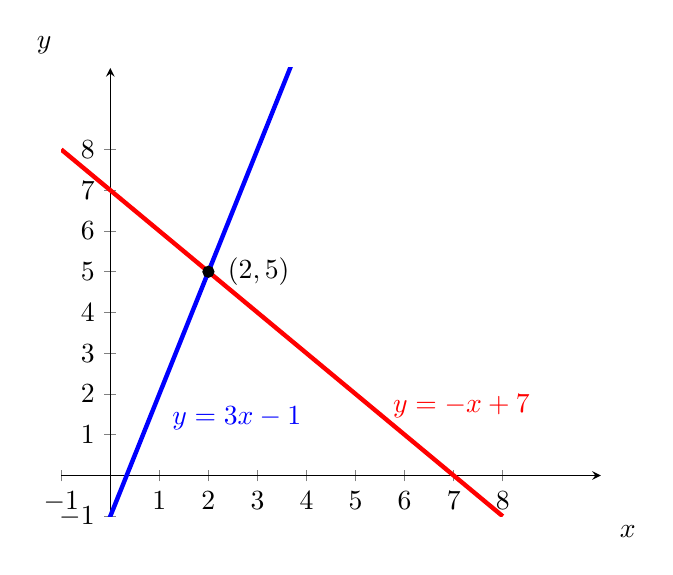
\begin{tikzpicture}[scale=1]
  \begin{axis}[
    axis lines=middle,
    xlabel={$x$},
    ylabel={$y$},
		xlabel style={at={(axis description cs:1.05,0)},anchor=north},
    ylabel style={at={(axis description cs:0,1.05)},anchor=east},
    xmin=-1, xmax=10,
    ymin=-1, ymax=10,
    xtick={-1,0,...,8},
    ytick={-1,0,...,8},
    samples=2,
  ]
  \addplot[blue, ultra thick, domain=-1:8]{3*x - 1} node[pos =.2, label={right:$y = 3x - 1$}] {};
  \addplot[red, ultra thick, domain=-1:8]{-x + 7} node[pos =.7, label={right:$y = -x + 7$}] {};
  \addplot[mark=*] coordinates {(2,5)} node[label={right:$(2, 5)$}] {};
  \end{axis}
\end{tikzpicture}
\end{center}

Finding an intersection of two lines graphically is not always easy or practical; therefore, we will now learn to solve these problems algebraically.

At the point where two lines intersect, the $x$ and $y$ values for both lines are the same. So in order to find the intersection, we either let the $x$-values or the $y$-values equal.

If we were to solve the above example algebraically, it will be easier to let the $y$-values equal. Since $y = 3x - 1$ for the first line, and $y = -x + 7$ for the second line, by letting the $y$-values equal, we get:

\begin{align*}
3x - 1 &= -x + 7 \\
4x &= 8 \\
x &= 2
\end{align*}

By substituting $x = 2$ in any of the two equations, we obtain $y = 5$. Hence, the solution is $(2, 5)$.
\end{solution}


\subsection{Solving Systems of Equations: The Elimination Method}

A common algebraic method used to solve systems of equations is called the elimination method. The objective is to eliminate one of the two variables by adding the left and right sides of the equations together. Once one variable is eliminated, we have an equation with only one variable that can be solved. Finally, by substituting the value of the variable that has been found in one of the original equations, we can get the value of the other variable.

\begin{example}
Find the intersection of the lines $2x + y = 7$ and $3x - y = 3$ by the elimination method.
\end{example}

\begin{solution}
We add the left and right sides of the two equations:

\begin{align*}
2x + y &= 7 \\
3x - y &= 3 \\
5x &= 10 \\
x &= 2
\end{align*}

Now we substitute $x = 2$ into any of the two equations and solve for $y$:

\begin{align*}
2(2) + y &= 7 \\
4 + y &= 7 \\
y &= 3
\end{align*}

Therefore, the solution is $(2, 3)$.
\end{solution}

\begin{example}
Solve the system of equations $x + 2y = 3$ and $2x + 3y = 4$ by the elimination method.
\end{example}

\begin{solution}
If we add the two equations directly, none of the variables are eliminated. However, the variable $x$ can be eliminated by multiplying the first equation by $-2$ and leaving the second equation unchanged:

\begin{align*}
-2x - 4y &= -6 \\
2x + 3y &= 4 \\
-y &= -2 \\
y &= 2
\end{align*}

Substituting $y = 2$ into $x + 2y = 3$, we get:

\begin{align*}
x + 2(2) &= 3 \\
x + 4 &= 3 \\
x &= -1
\end{align*}

Therefore, the solution is $(-1, 2)$.
\end{solution}

\begin{example}
Solve the system of equations $3x - 4y = 5$ and $4x - 5y = 6$.
\end{example}

\begin{solution}
This time, we multiply the first equation by $-4$ and the second by $3$ before adding (the choice of numbers is not unique):

\begin{align*}
-12x + 16y &= -20 \\
12x - 15y &= 18 \\
y &= -2
\end{align*}

By substituting $y = -2$ into any one of the equations, we get:

\begin{align*}
3x - 4(-2) &= 5 \\
3x + 8 &= 5 \\
3x &= -3 \\
x &= -1
\end{align*}

Hence, the solution is $(-1, -2)$.
\end{solution}

\subsection{Supply, Demand, and the Equilibrium Market Price}

In a free market economy, the supply curve for a commodity is the number of items of a product that can be made available at different prices, and the demand curve is the number of items the consumer will buy at different prices. As the price of a product increases, its demand decreases, and supply increases. On the other hand, as the price decreases, the demand increases, and supply decreases. The equilibrium price is reached when the demand equals the supply.

\begin{example}
The supply curve for a product is given by $y = 3.5x - 14$, and the demand curve for the same product is given by $y = -2.5x + 34$, where $x$ is the price and $y$ is the number of items produced. Find the following:
\begin{enumerate}
  \item How many items will be supplied at a price of \$10?
  \item How many items will be demanded at a price of \$10?
  \item Determine the equilibrium price.
  \item How many items will be produced at the equilibrium price?
\end{enumerate}
\end{example}

\begin{solution}
\begin{enumerate}
  \item To find the number of items supplied at a price of \$10, we substitute $x = 10$ into the supply equation $y = 3.5x - 14$. Therefore, $y = 3.5(10) - 14 = 21$ items will be supplied.
  
  \item To find the number of items demanded at a price of \$10, we substitute $x = 10$ into the demand equation $y = -2.5x + 34$. Therefore, $y = -2.5(10) + 34 = 9$ items will be demanded.
  
  \item To determine the equilibrium price, we set the supply equal to the demand:
  \[3.5x - 14 = -2.5x + 34\]
  Solving for $x$:
  \[6x = 48\]
  \[x = 8\]
  So, the equilibrium price is $x = 8$.
  
  \item To find how many items will be produced at the equilibrium price, we substitute $x = 8$ into either the supply or the demand equation. Using the supply equation, we get $y = 3.5(8) - 14 = 14$ items will be produced.
\end{enumerate}

The graph shows the intersection of the supply and demand functions and their point of intersection, $(8, 14)$.


\begin{center}
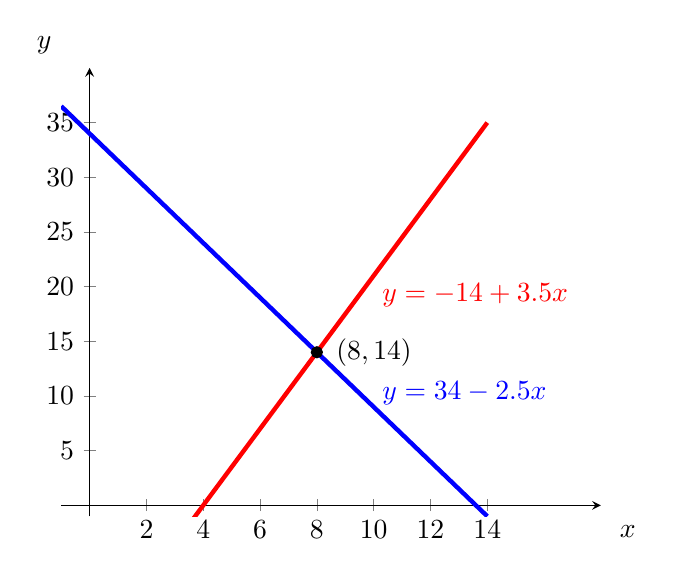
\begin{tikzpicture}[scale=1.0]
  \begin{axis}[
    axis lines=middle,
    xlabel={$x$},
    ylabel={$y$},
		xlabel style={at={(axis description cs:1.05,0)},anchor=north},
    ylabel style={at={(axis description cs:0,1.05)},anchor=east},
    xmin=-1, xmax=18,
    ymin=-1, ymax=40,
    xtick={0,2,...,14},
    ytick={0,5,...,35},
    samples=2,
  ]
  \addplot[blue, ultra thick, domain=-1:14]{34-2.5*x} node[pos =.7, label={right:$y = 34-2.5x$}] {};
  \addplot[red, ultra thick, domain=-1:14]{-14+3.5*x} node[pos =.7, label={right:$y = -14+3.5x$}] {};
  \addplot[mark=*] coordinates {(8,14)} node[label={right:$(8,14)$}] {};
  \end{axis}
\end{tikzpicture}
\end{center}

\end{solution}

\subsection{Break-Even Point}

In a business, profit is generated by selling products. If a company sells $x$ number of items at a price $P$, then the revenue $R$ is the price multiplied by the number of items sold: $R = P \cdot x$. The production costs $C$ are the sum of the variable costs and the fixed costs, often written as $C = mx + b$, where $x$ is the number of items manufactured.

\begin{itemize}
  \item The slope $m$ is called the marginal cost and represents the cost to produce one additional item or unit.
  \item The variable cost, $mx$, depends on how much is being produced.
  \item The fixed cost $b$ is constant and does not change regardless of production quantity.
\end{itemize}

Profit is equal to revenue minus cost: $Profit = R - C$. A company makes a profit if the revenue is greater than the cost, and there is a loss if the cost is greater than the revenue. The point on the graph where the revenue equals the cost is called the break-even point, and at this point, the profit is $0$.

\begin{example}
If the revenue function of a product is $R = 5x$ and the cost function is $C = 3x + 12$, find the following:
\begin{enumerate}
  \item If $4$ items are produced, what will the revenue be?
  \item What is the cost of producing $4$ items?
  \item How many items should be produced to break even?
  \item What will be the revenue and cost at the break-even point?
\end{enumerate}
\end{example}

\begin{solution}
\begin{enumerate}
  \item To find the revenue when $4$ items are produced, we substitute $x = 4$ in the revenue equation $R = 5x$, and the answer is $R = 20$.
  \item To find the cost of producing $4$ items, we substitute $x = 4$ in the cost equation $C = 3x + 12$, and the answer is $C = 24$.
  \item To determine the number of items required to break even, we set the revenue equal to the cost:
  \[5x = 3x + 12\]
  Solving for $x$:
  \[2x = 12\]
  \[x = 6\]
  So, $6$ items should be produced to break even.
  \item At the break-even point, when $x = 6$, we can substitute $x = 6$ in either the revenue or the cost equation to find that both revenue and cost are equal to $30$. Therefore, the revenue and cost at the break-even point are both $30$.
\end{enumerate}

The graph below shows the intersection of the revenue and cost functions and their point of intersection, $(6, 30)$.
\end{solution}

\begin{center}
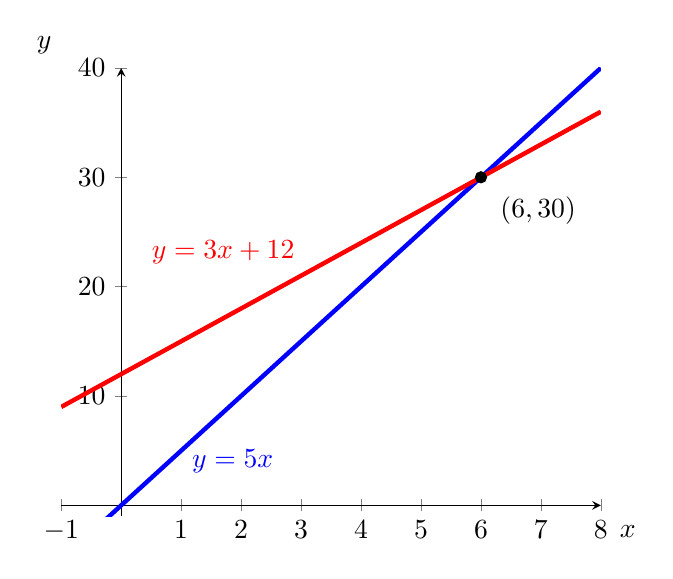
\begin{tikzpicture}[scale=1.0]
  \begin{axis}[
    axis lines=middle,
    xlabel={$x$},
    ylabel={$y$},
		xlabel style={at={(axis description cs:1.05,0)},anchor=north},
    ylabel style={at={(axis description cs:0,1.05)},anchor=east},
    xmin=-1, xmax=8,
    ymin=-1, ymax=40,
    xtick={-1,0,...,8},
    ytick={0,10,...,40},
    samples=2,
  ]
  \addplot[blue, ultra thick, domain=-1:8]{5*x} node[pos =.2, label={right:$y = 5x$}] {};
  \addplot[red, ultra thick, domain=-1:8]{3*x + 12} node[pos =.3, yshift=4mm, label={above:$y = 3x+12$}] {};
  \addplot[mark=*] coordinates {(6,30)} node[label={below right:$(6, 30)$}] {};
  \end{axis}
\end{tikzpicture}
\end{center}

